%!TEX root = ../thesis.tex
%Adding the above line, with the name of your base .tex file (in this case "thesis.tex") will allow you to compile the whole thesis even when working inside one of the chapter tex files
%: ----------------------- introduction file header -----------------------
\chapter{Introduction}
\label{chap:1}

The Sun has long been the focus of humanity's curiosity. Throughout history it has been the harbinger of new religions, philosophies, and sciences. It has changed our understanding of our place in the Universe and allowed us to push forward the frontiers of stellar astronomy. Although our understanding of the Sun is nowadays more advanced, the curiosity we hold for it has not changed since the very early humans.
Now, we understand the Sun is a star similar to any other in its class, currently going through a relatively unchanging 11 year cycle of activity that is extremely rich in physical complexity. The study of such complex phenomena has yielded immeasurable advances in many areas of physics such as spectroscopy, plasma physics, magnetohydrodynamics (MHD), particle physics, to name but a few. Although some of these sciences have grown over decades (or even centuries) they are still incomplete. I hope this theses, in some small way, will contribute to the continuing growth of these sciences and to the understanding of our nearest star.


%Here is the introduction of the thesis, complete with a few references  \citep{sagan1997demon, prothero2007evolution}.  Section \ref{sec:1} contains Equation \ref{eqn:1}, Section \ref{sec:2} has Figure \ref{fig:1} and Section \ref{sec:3} has Table \ref{tab:1}. Chapter \ref{chap:2} has pretty much nothing in it.

\section{The Sun}\label{sec:1}

The Sun is our nearest star, located $1.49\times10^6$\,km from Earth at the centre of our solar system. Located on the main sequence of the Hetzpring-Russel (HR) diagram, it has a spectral class of G2V, with a luminosity of $L_{\odot}=(3.84\pm 0.04)\times10^{26}$\,W, mass of $M_{\odot}=(1.989\pm0.0003)\times10^{30}$\,kg and radius of $R_{\odot}=(6.959\pm0.007)\times10^8$\,m \citep{foukal2004}. It was born approximately $4.6 \times 10^9$\,years ago when a giant molecular cloud underwent gravitational collapse and began hydrogen nuclear fusion at its centre (reference). The energy produced from this fusion resulted in enough pressure to counteract gravitational contraction and bring about a hydrostatic equilibrium, allowing the young star to reach a stability that is sustained today. It is estimated the Sun will maintain this stability for another 5 billion years, at which point, it will move off the main sequence and into a red giant phase. During this later part of its life, it will grow in size to 100 times its current radius and begin nuclear burning of heavier elements such as carbon and oxygen. Once carbon burning in the core has ceased it can no longer sustain nuclear fusion of heavier elements, resulting in a gravitational instability that will eventually lead to a stellar nova. This nova will result in the loss of the outer envelopes and ultimately the Sun's death, leaving behind a compact and dense white-dwarf.

Until such time, the Sun will remain on the main sequence in a regular state of hydrogen fusion in its core. The energy released during this process is the ultimate source of light and all energetic activity that we observe from Earth and beyond. Before we can understand how this energy manifests in the solar atmosphere as a variety of energetic phenomena, it is important to understand how the energy is generated and transported through its interior and finally released into its atmosphere and interplanetary space.

\subsection{Solar Interior}\label{sec:10}

The theoretical development on how the solar interior is structured and how it behaves has been through what is known as the \textquoteleft standard solar model' or SSM. The SSM is a grouping of theories that described how the Sun was formed, how it maintains its stability, how it generates energy, and how this energy is transported through its interior and released at the surface. Much of the major developments of this theory have been in the 20th century, due mainly to the pioneering experiments in solar neutrino physics and helioseismsology. Hence, the development of the SSM has mainly been through a refinement of the theory based on these observational fields. Although the SSM has increased in sophistication, its four main aspects remain the most general framework for describing the behavior of the solar interior.

The SSM firstly states that the Sun was born from the gravitational collapse of a primordial gas of hydrogen, helium, and traces of other heavy elements. Secondly, it maintains its structural stability via a hydrostatic equilibrium such that the gravitational force is balanced by a pressure gradient ($\grad{P}=-\rho g$) at each radial distance inside the star. The third main aspect of the SSM involves the source of the Sun's energy. Much of the early ideas proposed during the 19th century involved some form of chemical reaction or energy released during a slow gravitational contraction. However, during the first half of the 20th century the theory that the Sun is at least as old as the Earth began to come into focus. The idea of the Sun being more than 4.5 billion years old prompted the question of what energy source could sustain the Sun's luminosity for such a length of time. It was soon realised that thermonuclear fusion must be the source of such energy, and, as a result, it should be possible to observe the neutrino products of this fusion. Hence, starting in the 1950s a number of pioneering neutrino physics experiments were developed in an attempt to detect solar-generated neutrinos at Earth. These pioneering experiments, as well as there more sophisticated counterparts today, confirm much of the theories on solar core energy generation.

From the 1950s onwards there has been a confirmed detection of neutrinos generated in a hydrogen fusion process, namely the proton-proton or \textquoteleft pp'-chain, in the solar core. In this process, four protons are fused to form a helium nucleus. This can occur in a variety of ways, but at the Sun's core temperature of 15 MK, the dominant reaction is the pp 1 chain given by
\begin{equation}
^{1}_1\mathrm{H} + ^{1}_1\mathrm{H} \rightarrow ~^{2}_1\mathrm{H} + e^{+}  + \nu_e
\end{equation}
\begin{equation}
^{2}_1\mathrm{H} + ^{1}_1\mathrm{H} \rightarrow ~^{3}_2\mathrm{He} + \gamma
\end{equation}
\begin{equation}
^{3}_2\mathrm{He}+^{3}_2\mathrm{He} \rightarrow ~^{4}_2\mathrm{He} + 2^{1}_1\mathrm{H}
\end{equation}
where $^{1}_1\mathrm{H}$ is a hydrogen nucelus, $^{2}_1\mathrm{H}$ is deuterium, $^{3}_2\mathrm{He}$ is tritium, $^{4}_2\mathrm{He}$ is helium, $e^{+}$ is a positron, $\nu_e$ is an electron neutrino, and $\gamma$ is a gamma ray photon. Reactions (1.1) and (1.2) must happen twice for (1.3) to occur. Taking this into account, the entire process may be summarised as 
\begin{equation}
4 ^{1}_1\mathrm{H}  \rightarrow ~^{4}_2\mathrm{He} + 2e^{+} + 2\nu_e + 2\gamma
\end{equation}
liberating $4.2\times10^{-12}$J of energy, with $\sim2.4$\% of the energy carried away by the neutrinos. This particular form of the pp-chain (pp 1) occurs in 86\% of the cases \citep{turk2011}. However, there are other reactions capable of producing He from H catagorized into pp II, pp III etc, which each involve production of $^7_4$Be and $^8_5$B. The initial neutrino detections at Earth were the result of the pp III reaction which involves the creation of $^8_5$B, followed by a decay to $^8_4$Be, a positron, and an electron neutrino \citep{davis1968}. These early detections and the results of more recent experiments such as the SuperKamiokande \citep{fukuda1998} show that the expected neutrino flux given by the standard solar model is smaller than the observed. This deficit in in neutrino flux observations became the famed \textquoteleft solar neutrino problem' during the 1970s. 
One of the proposed explanations for the process was via an oscillation of the neutrino amongst three sets of 'flavors' i.e., the neutrino can be either an electron $\nu_e$, muon $\nu_{\mu}$, or tau $\nu_{\tau}$ neutrino. With the original detectors only being able to detect the $\nu_e$, this would result in a flux deficit (non-detection of $\nu_{\mu}$ and $\nu_{\tau}$). This oscillation amongst three flavors was given the name the \textquoteleft MSW effect' after \citet{mikheev1986} and \citet{wolfenstein1978}, and later confirmed experimentally by the SuperKamionkande experiment.

The neutrino experiments together with the standard solar model SSM provide much of what we know about the solar energy generation and the solar core. They imply a temperature of $15.6\times10^6$K and density of $1.48\times10^5$\,kg\,m$^{-3}$ at solar centre, and also confirm the existence of a variety of pp reactions (pp 1 to pp IV), and some level of Carbon-Nitrogen-Oxygen (CNO) fusion process. These fusion processes occur over $0.0-0.25\,R_{\odot}$ (Figure~\ref{fig:solar_atmosphere}), which defines the solar core. Outside the core the temperature drops to a value such that fusion ceases. While thermonuclear fusion is the third aspect of the SSM involves the generation of solar energy, the fourth aspect involves exactly what happens to this energy once it is generated i.e., it describes an energy transport mechanism.


Beyond $0.25\,R_{\odot}$ the temperature drops to 8 MK, such that fusion stops but only free protons and electrons exist. In this environment, the photons continuously scatter off free particles, undergoing a random walk toward the surface over a distance of $0.25-0.7\,R_{\odot}$. This region is known as the radiative zone and has densities of $2\times10^4-2\times10^2$\,kg\,m$^{-3}$, resulting in a small photon mean free path (mfp) of $9.0\times10^{-4}$\,m. The photons proceed towards the solar surface over a very long time scale, taking on the order of $10^{5}$ years to traverse this region \citep{mitalas1992}. If radiative energy transport occurs, it will result in the following temperature gradient
\begin{equation}
\frac{dT}{dr} = -\frac{3}{16 \sigma}\frac{\kappa \rho}{T^3}F_{rad}
\end{equation}

%Note the above equation is actually a diffusion equation for radiation. Take the divergence of both sides and you have $\grad\dotF = \kappa^'\grad^2 T$, with $\kappa^'$ being the diffusion coefficient given by $\kappa^i=\frac{16\pi\sigmaT^3}{3\kappa \rho}$ e.g., the opacity controls to mean free path, and hence the diffusion of photons.


where $\sigma$ is the Stefan-Boltzman constant, $\kappa$ is the mass extinction coefficient (opacity per unit mass), $\rho$ is mass density, $T$ is temperature, and $F_{rad}$ is the outward radiative flux. This implies that for a particular outward flux, if the opacity increases, a steeper temperature gradient is required to maintain such a flux. At $0.7\,R_{\odot}$ the temperature drops to 1\,MK allowing protons to capture electrons into a bound orbit. The existence of electrons in atomic orbit results in a dramatic increase in opacity of the plasma \citep{turk2011} and hence the temperature gradient increases. The increased temperature gradient required to sustain the energy flow may lead to the onset of a convective instability beyond $0.7\,R_{\odot}$ toward the solar surface. This instability will occur if the temperature gradient in the star is steeper than the adiabatic temperature gradient
\begin{equation}
\Bigg|\frac{dT}{dr}\Bigg|_{star} > \Bigg|\frac{dT}{dr}\Bigg|_{adiabatic}
\end{equation}
This is known as the Schwarzchild criterion, and it is fulfilled from $0.7-1\,R_{\odot}$ $-$a region known as the convection zone. The temperature and density drop as height increases and finally reaches T$\sim$$6000$\,K and mass densities of $\rho\sim1\times10^{-5}$\,kg\,m$^{-3}$. Although no complete theoretical treatment of convection exists, mixing length theory and hydrodynamical modeling are used to determine how convection occurs in the solar interior. Convection ceases at $1\,R_{\odot}$, where the environment makes a sudden transition to convectively stability. At this point the opacity drops and energy is released in the form of radiation, demarcating the start of the solar surface, known as the photosphere. 

\begin{figure}[!t]
\begin{center}
\includegraphics[trim = 0cm 0.5cm 0cm 0cm, width=1.0\textwidth]{images/solar_atmosphere}
\caption{The internal structure of the Sun, including the core, radiative zone, and convective zone.  Also shown is the structure of the its atmosphere, including the photosphere, chromosphere, and corona. The layers of the solar atmosphere are usually demarcated by temperature changes as height above the solar surface increases. The temperature ranges from $\sim$6000\,K in the photosphere to above 1\,MK in the corona.}
\label{fig:solar_atmosphere} 
\end{center}
\end{figure}

% Yuhong Fan, Living Reviews. "Because of the rapid decrease of the various scale heights in the top layer of the solar convection zone which demands increasing numerical resolution, it is not yet feasible to perform 3D MHD simulations that extend from the bottom of the convection zone all the way to the photosphere."

Much of what we know about the depth, temperature, and density of the convection zones come from a fine-tuning of the standard solar model, such that the model reproduces observations from neutrino and helioseismology experiments. In fact helioseismology alone can indicate great detail of the internal structure of the Sun. This field makes use of the fact the Sun acts as a resonator for acoustic waves which manifest as detectable oscillations in the doppler shift of photospheric Fraunhofer lines. These acoustic waves are referred to as pressure or p-modes, and a variety of wavelengths exist. Wavelengths that are an integer multiple of of the solar cavity may exist as standing wave modes. Such wave modes have a period of approximately 5 minutes \citep{turk2011}. 

\begin{figure}[!t]
\begin{center}
\includegraphics[trim = 0cm 0.5cm 0cm 0cm, width=1.0\textwidth]{images/differential_rot.png}
\caption{Helioseismological determination of interior rotation rate in nanoHertz (nHz) as a function solar radius, starting from solar centre ($r=0.0$) to surface ($r=1.0$). The separate symbols show different latitudes, from $0^{\circ}$ to $75^{\circ}$. The data show that the interior rotates differentially down to $\sim$$0.7\,R_{\odot}$. The dashed line demarcates the boundary between solid body rotation and differential rotation \citep{thompson2003}.}
\label{fig:diff_rot} 
\end{center}
\end{figure}


The shorter wavelengths in the mode propagate into the solar convection zone and experience a total internal reflection at a shallow depth, while longer wavelengths can penetrate into much deeper layers. Hence depending on the period observed, the oscillations provide a probe of the internal thermodynamic properties at a particular level. Once such property closely monitored is the sound speed, which is seen to match the predicted sound speed based on the standard model. However, the observation and prediction show the biggest deviation at a depth of $0.3\,R_{\odot}$, which is the region where the radiative zone transitions to the convective zone. This obviously implies that SSM is lacking in its description of how the solar interior is stratified at this depth. This partly due to the fact the SSM does not take into account differential rotation. The solar surface rotates faster at the equator than it does at the poles i.e., angular velocity is stratified with latitude. Helioseismology has revealed that such differential rotational continues to the bottom of the convection zone. In the deeper radiative zone and core the Sun rotates as a solid body see Figure~\ref{fig:diff_rot}. There is a dramatic change in the internal dynamics when transitioning from convective to radiative zones. 

As predicted by sound speed measurements and differential rotation, the region sandwiched in between radiative and convective zones is and extremely important boundary. It is known as the tachocline, and the dynamics of this thin layer is believed to play and extremely important role in the generation and evolution of the solar magnetic field \citep{thompson2003}.




\subsection{Solar Magnetic Field and Dynamo}\label{sec:11}

The solar magnetic field is the ultimately source of all energetic activity in the its atmosphere. At solar activity minimum the solar magnetic field has a poloidal dipolar structure, with the polar axes generally being coincident with the rotational axes. However as the the activity cycle progresses towards a maximum, the field gains a strong toroidal component, making it far more dynamic and complex. This complex toroidal component manifests at the surface as sunspots, hence the number of sunspots on disk has been used as a proxy for the activity cycle for over 100 years, often showing an approximate 11 year periodicity (Figure~\ref{fig:butterfly}, bottom panel). At the beginning of the cycle sunspots tend to appear on disk with a latitudinal distribution of $\pm30^{\circ}$ of the equator. As the cycle progresses, sunspots appear at lower and lower latitude (known as Sp\"{o}rer's law), until they eventually disappear at the end of a cycle. Sunspot latitude with respect to time is shown in Figure~\ref{fig:butterfly}, top panel, and is known as the butterfly diagram.

Sunspots in there simplest case emerge as a dipole structure, with the leading spot being closer to the equator, such that the dipole is titled relative to the solar equator (Joy's law). In a given hemisphere, the leading sunspot and trailing spot have opposite polarities, with the polarities reversed in the other hemisphere  (Hayle's law). The trailing polarity can often be more fragmented and dispersed that the leading polarity. Despite sunspots generally having a dipolar structure, spot groups can be far more complex, having a multipolar structure (this will be described more later).

Over the course of a solar cycle, the sun changes polarity (at the time of sunspot maximum). For example, an overall dipolar configuration of North-South will become South-North, another cycle will bring it back to N-S once more. While the activity cycle usually last 11 years, one full magnetic cycle has a period of 22 years.


\begin{figure}[!t]
\begin{center}
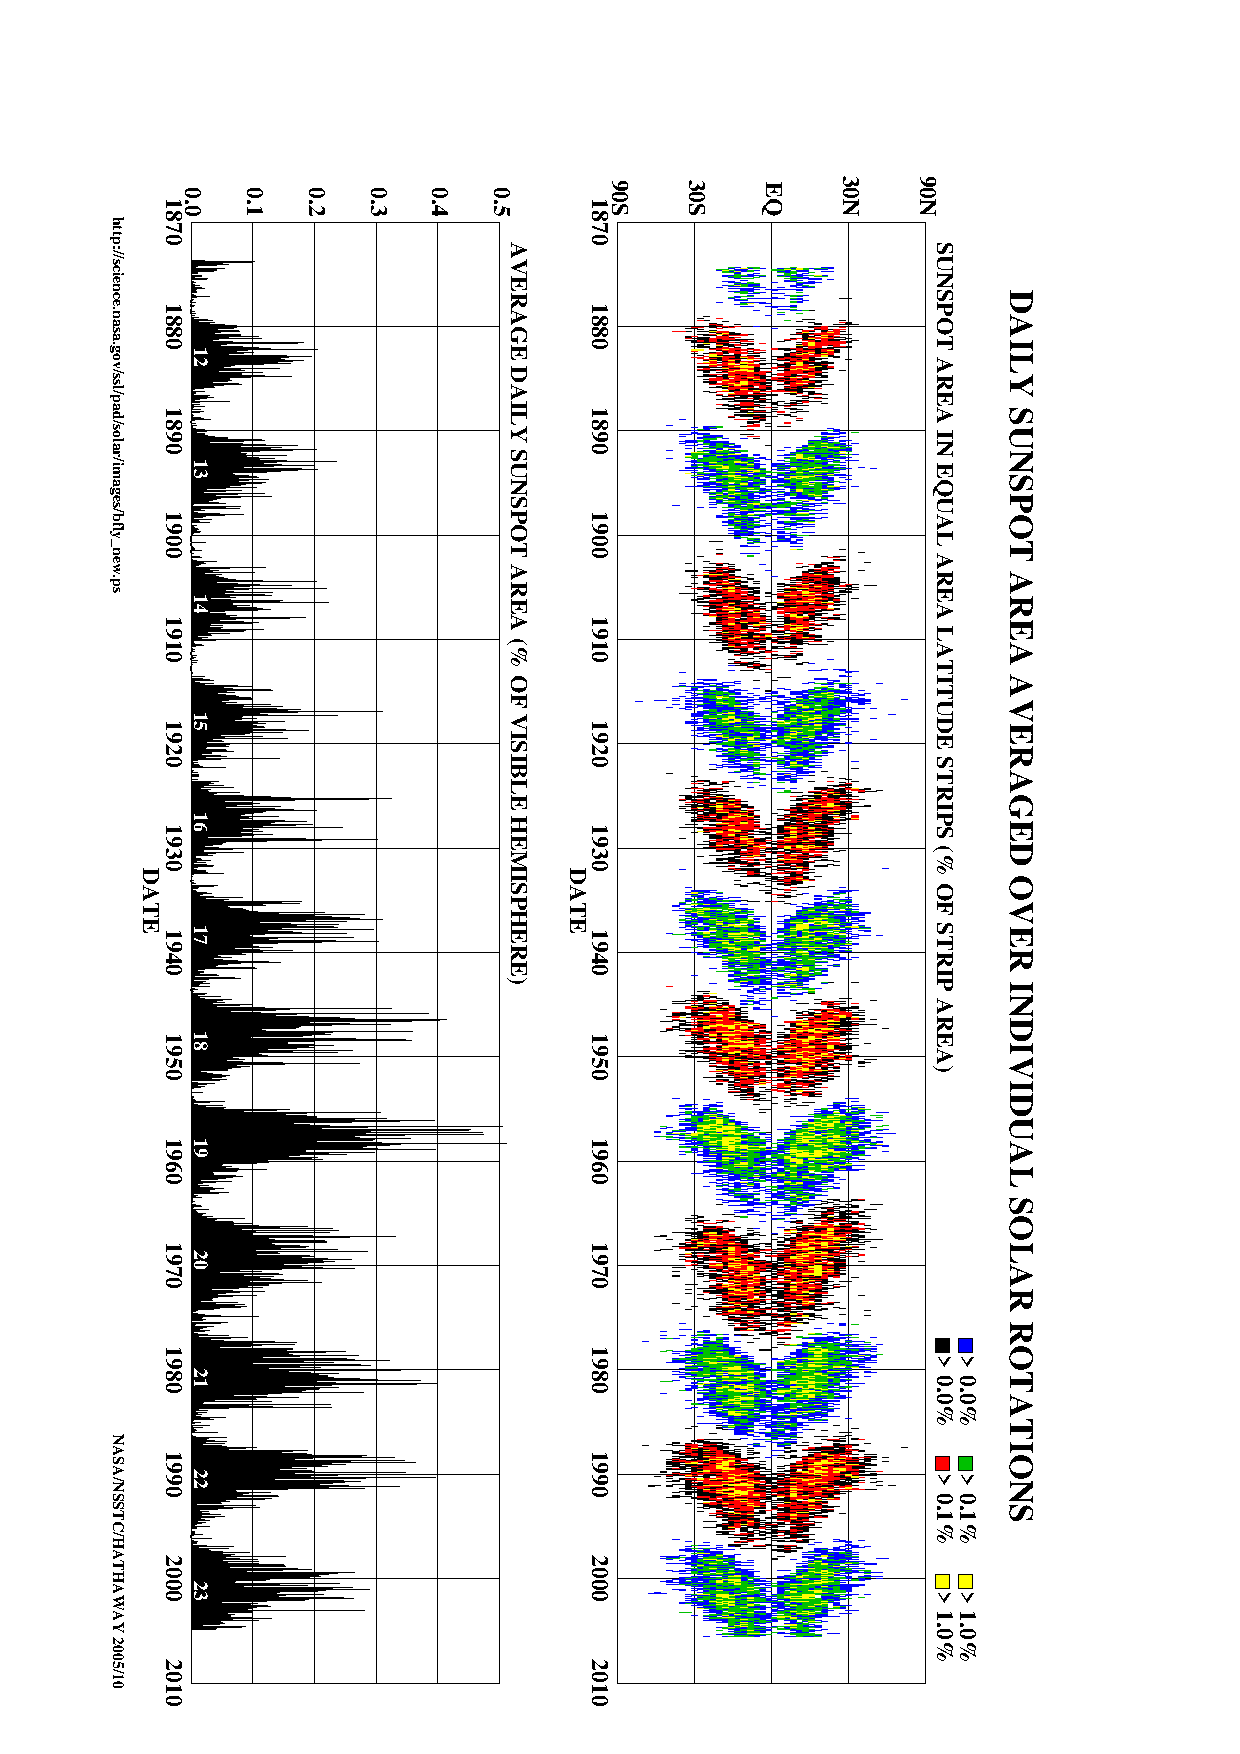
\includegraphics[scale=0.55, trim =1cm 1cm 0cm 3cm]{images/bfly_new.pdf}
\caption{Top: The latitude of sunspots as a function of time. During the rise phase of each cycle the sunspots have a latitudinal distribution of $\pm30^{\circ}$ from the equator.  As the solar cycle progresses, sunspots emergence takes place at an increasingly lower latitude. Bottom: Sunspot area as a function of time. The approximate 11 year periodicity is clearly shown.}
\label{fig:butterfly} 
\end{center}
\end{figure}


\begin{figure}[!h]
\begin{center}
\includegraphics[]{images/Babcock}
\caption{Differential rotation and flux freezing result in the poloidal dipolar magnetic field, generated by dynamo action, to be dragged around in a toroidal direction, an action known as the omega effect. Buoyancy of the field lines results in them rising and twisting, known as the alpha effect, eventually surfacing to become bipolar fields that extend far into the corona.}
\label{fig:Babcock} 
\end{center}
\end{figure}

The complex behavior of the solar magnetic field over an 11 year activity cycle, during which the dipole flips, is generally explained by solar dynamo theory. This involves large-scale flow patterns of the solar interior that act to both induct and diffuse the magnetic field such that it produces the familiar 11 year magnetic activity cycle. Magnetohydrodynamics (MHD) is employed such that the magnetic induction equation and velocity field equation (equation of motion) are solved in numerical models to produce a toroidal field from a poloidal one, a process known as the $\Omega$-effect. The theories must adhere to the constraints provided by observations of the sunspot cycle (Sp\"{o}rer's, Joy's, and Hale's laws), and also helioseismology observations of how the interior is structured.


\citet{babcock1961} first proposed a mechanism whereby the differential rotation of the solar convection zone tends to drag the field from a poloidal position into a toroidal one, eventually winding the field into a a stressed state, see Figure~\ref{fig:Babcock}. The main storage of this wound field is in the region below the convection zone known as the tachocline. This region is known as an 'overshoot' layer, in which descending convective flows are a trapped due the subadiabicity of the region (convectively stable). This stability allows field to be built up and stored into complex magnetic structures. Parts of this structure may form a twisted magnetic 'flux-rope', and due to it's excess magnetic pressure, it becomes convectively unstable and begins to rise. During this rise a Coriolis force has a tendency to tilt into a north-south orientation and eventually penetrate through the solar surface and into the atmosphere, known as the $\alpha$-effect (the tilt from Coriolis effects explains Joy's law). Dynamo theory attempts to explain the $\Omega$-effect wrapping and build up of toroidal flux in the solar interior via inductive plasma flows \citep{charbon2010}, particularly using the observed flow structure from helioseismology. Further MHD of convective instabilities is employed to describe the $\alpha$-effect rise of flux systems into the solar atmosphere from the stably convective tachcoline/overshoot layer. This is very much a study in itself, and describes the eventual formation coronal active regions from sub-photospheric flux-systems \citep{fan2009}. 


\subsection{Solar Atmosphere}\label{sec:12}

The solar atmosphere begins above the visible surface of the sun, known as the photosphere. At this point, the Sun become optically thin to visible radiation and light escapes from this surface. Beyond this visible surface is the solar chromosphere, the corona, which eventually becomes the solar wind. Each of these layers is home to a complex array of phenomena, and each layer with it's accompanying attributes is described here.


\subsubsection{Photosphere}\label{sec:121}

As mentioned the photosphere begins where the atmosphere become optically thin. \textquoteleft Visible light' in this instance is usually taken to mean light with a wavelength of 5000\,\AA, hence the emergent light from the photosphere is taken to come from the surface at which $\tau_{5000}=2/3$. This is a consequence of the Eddington-Barbier approximation, and says that emergent flux $F_{\nu}$ from the photosphere is given by

\begin{equation}
F_\nu = \pi B_\nu(\tau=2/3)
\end{equation}
e.g., the emergent flux is given by $\pi$ times blackbody intensity at an optical depth of 2/3, where blackbody intensity $B_\nu$ is given by Planck's law 
\begin{equation}
B_\nu = \frac{2h\pi\nu^3}{c^2}\frac{1}{\mathrm{exp}(h\nu/k_BT)-1}
\end{equation}
where $h$ is Planck's constant, $\nu$ is frequency, $c$ is the speed of light, $k_B$ is Boltzmann's constant, and $T$ is temperature. Integrated over frequency this results in $F = \sigma T^4(\tau=2/3)$, where the frequency integrated flux is proportional to the temperature at $\tau=2/3$, hence the effective temperature of solar blackbody radiation is $T_{eff}=T(\tau=2/3)=5800$\,K. Solar radiation at visible wavelengths is most closely characterised by a blackbody of temperature 5800 K, although the brightness temperature $T_B$ the solar photosphere can deviate from this value, since not all frequencies emerge from the same optical depth.

The visible appearance of the photosphere reveals a small scale granular structure, with granules of typical size scale of 1000\,km with a lifetime of 5-10 minutes. The granules typically show bright centers surrounded by darker intergranular lanes. Doppler measurements reveal that granule centres have a positive (upward) velocity of up to $\sim1$\,km\,s$^{-1}$, with intergranular lanes having a negative (downward) velocity. Such upward and downward flow reveals that granulation at the photosphere are the surface manifestation of convective activity in the deeper layers of the sun, although the size scales of granules are much smaller than the convective plumes believed to permeate the convection zone. As well as the conspicuous granulation at the photospheric surface there is also a much larger scale \textquoteleft super-granulation' which has much the same mechanism as the granules e.g, upflows at granule centre and downflows at the edges in the granular network. The flow speeds are much slower with typical speeds of $0.1$\,km\,s$^{-1}$. The have a much larger size of $10,000-30,000$\,km and longer lifetimes of several days. They have an important role in the build up and concentration of magnetic flux in the intergranular lanes. Apart from, granules and supergranules, the most conspicuous features of the photosphere are sunspots. As discussed in the previous section, these are the surface manifestation of concentrated magnetic flux that has penetrated from the solar convective zone into the solar atmosphere. The spots have a temperature of $\sim4000$\,K, which is cooler than the typical solar blackbody temperature of $5800$\,K. The spots have typical magnetic field strengths of on the order of kilo-Gauss, and have an important role to play in solar activity.


Although the the intensity of the Sun in the visible may be approximated closely by a blackbody continuum, there are also the presence of dark absorption or Fraunhofer lines in the spectrum. The most notable of which are the H$\alpha$ and Ca\Rmnum{2} H and K lines.  The presence of these lines reveals that cooler part of the photosphere must overly the hotter base at $\tau_{5000}=1$ \citep{phillips2008}. In fact, the variety of lines that are produced in the solar atmosphere (both emission and absorption) are used to determine the temperature and density stratification of the solar atmosphere.  That has most notably been done in the models of \citep{vernazza1981, fontenla1988, gabriel1976}, whereby a temperature and density profile of the solar atmosphere is used to calculate the emergent intensity, using radiative transfer theory. This temperature and density profile is adjusted until the the modeled emergent intensities match the observed ones. The results of this these models is shown in Figure~\ref{fig:val}. From this Figure we see that there is a temperature minimum at $\sim$500\,km above the photosphere where the temperature drops to $\sim$4400\,K. Beyond this point the temperature begins to rise again, eventually showing a rapid increase at $\sim$2000\,km. The region between the temperature minimum up the height at which temperature begins to rise rapidly is known as the chromosphere\footnote{These boundaries can vary, depending on the phenomenon observed e.g., spicules are chromospheric phenomenon which can extend far beyond the upper boundary of $\sim$2000\,km}. 

%About 15% of photospheric opacity is attributed to absorption features. The rest is H- opacity

\begin{figure}[!t]
\begin{center}
\includegraphics[scale=0.4]{images/VAL.png}
\caption{Temperature and density variation in the solar atmosphere constructed from the models of \citep{vernazza1981, fontenla1988, gabriel1976}, adopted from \citep{phillips2008}.}
\label{fig:val} 
\end{center}
\end{figure}


\subsubsection{Chromosphere}\label{sec:122}

As predicted by the models of \citep{vernazza1981, fontenla1988, gabriel1976}, at $\sim$500\,km above the $\tau_{5000}=1$ surface the temperature drops to a minimum of $\sim$4400\,K. Beyond this minimum the temperature begins to rise again, demarcating the beginning of the chromosphere. This layer of the atmosphere is generally accepted to extend to a height at which temperatures reach 20,000\,K, however temperatures as high as $\sim$$1\times10^5$\,K are sometimes attributed to chromospheric heights, hence it is observable at ultraviolet (UV) wavelengths as well as visible. 

The chromosphere is primarily observed through the the Fraunhofer H$\alpha$ and Ca\Rmnum{2} H and K lines. These lines in particular provide a good diagnostic of the chromospheric environment over a large height range since different sections of the lines are formed over various heights. By viewing the sun at or near the cores of the lines we may view different height s in the chromospheric part of the atmosphere. The chromosphere, when observed using the Ca lines, shows a highly non-uniform structured and structured appearance. The structure is made up of dark cells with a diameter of approximately 30,000\,km, with bright boundaries of the cells making up a network of bright features known as \textquoteleft the chromospheric network'. These network boundaries consisting of bright points are positions of near vertical magnetic field with a strength of 10\,Gauss. This chromospheric network is directly related to the supergranular structure as observed in the chromosphere i.e., the supergranular flows in the photosphere tend to transport field toward the boundaries of the network where they may coalesce and strengthen. These regions of strong magnetic field facilitate heating in the upper chromosphere and hence show up as regions of enhanced emission (by magnetic acoustic oscillations) in the centers of the Ca\Rmnum{2} K3, for example \citep{mcateer2002}. Enhanced emission in the internetwork regions (supergranule centres) show up as bright points when viewing Ca H2V and are now accepted to be formed by heat of the mid-low chromosphere by acoustic shocks \citep{carlsson1997}

Beyond the temperature minimum there is a broad temperature plateau between $\sim$$1000-2000$\,km, after which the temperature starts to increase dramatically. When the temperature reaches 20,000\,K the extremely prominent Ly-$\alpha$ emission line is formed, with a wavelength of 191.5\,nm, and this is accompanied by other prominent ultraviolet lines such as those of C \Rmnum{4}, formed at temperatures of $\sim$110,000\,K. Such high temperatures are generally considered to be outside the range of the chromosphere and are indicative of a thin layer of the atmosphere known as the transition region. This layer is on the order of a few hundred kilometers thick but has an extremely steep temperature gradient, carrying temperatures into the mega-Kelvin range. The region of the atmosphere with temperatures greater than $1\times10^{6}$\,K is known as the solar corona.

%Acoustic shocks heat the low-mid chromosphere in the internetwork region (supergranule centres) and show up as bright points when viewing Ca H2V lines. But the magnetic bright points (at the network boudnary) in higher altitude lines are thought to be upper chromosphere where MHD waves heat the environment, as evidenced by brightening in Ca K3 core. 

%It seems as though whether it's acoustic or magnetic heating depends on the lines (or position in the line) that we look at. If we see bright points in low altitude lines then is shocks. Bright points in high altitude lines correspond magnetic heating. 

%\begin{itemize}
%\item Appearance, Supergranular Network, Bright Points, Spicules, Filaments, Plage etc.
%\item Emission lines, H-alpha, CaII H \& K. 
%\item Temperature, Density, Opacity.
%\item Magnetic field strength.
%\end{itemize}

%Details in the chromosphere are imaged using the lines of H-alpha and Ca II H and K. These Fraunhofer lines are formed over a large range in heights.

%The H-alpha line is photoelectrically controlled, so the decrease in line intensity is to do with the source function being lower because of a lack of photospheric photons at that height the line centre 'samples

%Ca II  H and K is collisionally controlled so the decrease in line intensity is to do with the source function being lower because of the dropping temperature

%Different regions in the Ca II  H and K lines sample different heights in the photosphere/chromosphere. Tuning imagers to different parts of these lines allows imaging of chromosphere at different heights.

%Chromospheric lines not in the visible are the Mg h and k Fraunhofer lines, also collisionally controlled. There is also the Ly-alpha emission line, formed at 20,000 K, which is optically thin. There is C IV, formed at 110,000 K, at this point we are starting to sample to transition region.


%Note: Fraunhofer lines such as Calcium H and K are not as simple as a case of a cloud of cooler gas absorbing lines from a hot radiations source. The Fraunhofer lines are a consequence of the Eddington-Barbier Approximation i.e., that the emergent intensity is equal to the source function at an optical depth of 2/3. So in the centre of the line the opacity goes up and optical depth 2/3 is higher in the atmosphere where the plasma is cooler. Hence, the line is darker at the centre (due to the smaller source function at the cooler temperature).

\subsubsection{Corona}\label{sec:123}

The outermost layer of the solar atmosphere is known as the solar corona, beginning at $\sim$2500\,km above the photosphere. It has an electron number density of $10^{9}$\,cm$^{-3}$ at its base in quiet regions, decreasing to $10^{6}$\,cm$^{-3}$ at distance of $1\,R_{\odot}$ from the solar surface. The models of \citep{vernazza1981, fontenla1988, gabriel1976} reveal that beyond the transition region ($\sim$2500\,km) the temperature in the corona reaches well over $1\times10^{6}$\,K. Such high temperatures allow the formation of emission features that belong to highly ionized heavy elements, for example Fe \Rmnum{9}, up to as high as Fe \Rmnum{24}. The presence of these highly ionized species (and many others) show that the corona has temperatures in the $1-2$\,MK range in quiet regions, active regions may exhibit temperatures in the range of $2-6$\,MK, while coronal holes may be lower than 1\,MK. The temperatures of a flaring active region can be even higher than this, reaching tens of mega-Kelvin. The high temperatures and presence of highly ionized species of heavy elements means the corona is an emitter in the ultraviolet and X-ray. When viewed at these wavelengths, the corona appears highly structured, showing concentrations of bright loops known as active regions (Fig.~\ref{fig:aia171}).
\begin{figure}[!t]
\begin{center}
\includegraphics[scale=0.15]{images/aia_171}
\caption{Atmospheric Imaging Assembly\,171\,\AA\,image of the solar corona. Bright regions are strong concentrations of magnetic fields known as active regions (temperatures of $2-6$\,MK). Areas outside these regions are known as quiet sun (temperatures $1-2$\,MK).}
\label{fig:aia171} 
\end{center}
\end{figure}

Ultraviolet wavelengths allow observations of the very low corona, perhaps to only a few scale heights. However, the most extensive observations of the corona are in the visible, generally known as the 'white-light' corona. The corona's white-light radiation is primarily due to scattering of photospheric light by particles and dust grains. The component which is due to Thomson scattering by free electrons is known as the {\it Kontinuierlich} or K-corona. The spectrum of this light is same as the photospheric continuum except for the absence of Fraunhofer lines. These lines are 'washed-out' of the spectrum due to thermal Doppler broadening of the high-velocity free electrons on the corona. The emission is optically thin, so the intensity is due to the number of scattering agents along the line of site. The emission is also highly polarized, depending on he line of site of the observer (we will return to this important aspect later). The K-corona dominates white-light emission from low atmosphere to $\sim$4$R_{\odot}$. After this height, there is an increasing contribution from Rayleigh or Mie scattering from interplanetary dust grains, known as the the Fraunhofer F-corona. Since these dust grains move at a much slower velocity than the electrons, they do not wash out the Fraunhofer lines of the photospheric spectrum. The F-corona extend far beyond Earth and a can be viewed in the night sky as {\it Zodiacal light}.

Ultraviolet and white-light observations remain the primary method of imaging the low and extended corona, respectively. However, the corona is also a strong emitter across the entire radio wavelength range, from microwave to kilometric wavelengths. Indeed, metric wavelengths provide a method of imaging the quiet and thermal corona in an optically thick regime beyond $1\,R_{\odot}$, an ability that does not exist in white-light and UV observations. These radio observations can reveal much of the same features as other wavelengths (albeit at lower spatial resolution) such as bright emission of active regions and also coronal holes (Fig.~\ref{fig:lowfeq}).
\begin{figure}[t!]
\begin{center}
\includegraphics[scale=0.55]{images/low_freq_obs}
\caption{Low frequency observations of the solar atmosphere. Nan\,{c}ay Radioheliograph (NRH) 164MHz (top left), 327\,MHz (upper right), and 410\,MHz bottom left. Yohkoh Soft X-ray Telescope (SXT) image for comparison. Note the coronal holes in the SXT image is also in the 164 MHz image of NRH. The active regions are also bright at 327\,MHz and 410\,MHz \citep{lantos1999}}
\end{center}
\label{fig:lowfreq}
\end{figure}

The quiet corona at metric wavelengths is primarily an emitter of thermal Bremsstrahlung i.e., thermal electrons accelerating in the Coloumb electric fields of protons. The height at which metric radiation escapes from the corona depends on the Bremsstrahlung absorption process, known as free-free opacity and given by
\begin{equation}
\kappa_{ff} \sim \frac{n^2}{\nu^2T^{3/2}} 
\end{equation}
where $n$ is the electron number density, $\nu$ is the frequency of electromagnetic radiation, and $T$ is the temperature. Qualitatively, for a given frequency the density must drop below a certain value for the radiation to become optically thin and escape the solar atmosphere. In the radio band, even the highest frequency (microwaves) do not escape until densities drop to chromospheric values. Hence a microwave image of the sun will provide a direct observation of light escaping from the chromosphere. Reducing the frequency further still to the $10^{8}$Hz (metric wavelengths), the density must drop to coronal values before the free-free opacity is low enough for radiation to be optically thin. Hence, metric wavelength radiation escapes the solar atmosphere only in the outer corona. For example 150\,MHz imaging of the solar atmosphere may image an optically thick atmosphere out to a height of $\sim 0.5\,R_{\odot}$. The existence of an optically thick atmosphere at these wavelengths allows a direct probing of coronal temperatures at these heights. Using the solution to the radiative transfer equation
\begin{equation}
T_B = T_0e^{-\tau_{\nu}} + T_e(1-e^{-\tau_{\nu}})
\label{eq:rad_trans}
\end{equation}
where $T_B$ is the observed brightness temperature, $T_0$ is the background source brightness temperature, and $T_e$ is the electron temperature of a cloud of plasma between observer and source\footnote{Note that radio observations often use brightness and electron temperatures in place of specific intensity and the source function because radio observations are often calibrated via a load of known temperature}, we can separate the this equation into two regimes. Firstly,
in the optically thick regime $\tau_{\nu}>>1$ equation~\ref{eq:rad_trans} reduces to $T_B = T_e$, indicating that the brightness temperature is a direct measure of the electron temperature in solar atmospheric plasma. Secondly, in the optically thin regime $\tau_{\nu}<<1$, equation~\ref{eq:rad_trans} reduces to 
\begin{equation}
T_B = T_0(1-\tau_{\tau}) + T_e\tau_{\nu}
\end{equation}
Considering the case of no background source we see that for the optically thin regime $T_B = T_e\tau_{\nu}$ i.e., the brightness temperature is not a direct measure of the electron temperature, but is reduced by a factor of $\tau_{\nu}$. Note if the electrons are thermodynamic equilibrium then $T_e$ is simply the temperature of the plasma $T$, given by the Maxwell-Boltzmann distribution, meaning  a measure of brightness temperature allows a direct probing of the coronas thermal properties at this height. For example, a measure of brightness temperature at 100\,MHz will given $T_b\sim10^6$\,K. However, beyond 1\,GHz the corona becomes optically thin and brightness temperature then drops to $\sim10^{5}$\,K. 

It is also possible to observe non-thermal source in the solar atmosphere, especially during times of high activity. In the case of non-thermal radiation, $T_e$ is replaced by $T_{eff}$, the effective temperature, which is related to the average energy of the emitting particles $<E>=kT_{eff}$, where $k$ is Boltzmann's constant. In such a case, the brightness temperatures may be in excess of $10^{9}$\,K. These emissions are usually associated with flaring and eruptive activity and include gyrosynchrotron emission and plasma emission resulting. Since the observation of plasma emission is partly the subject of this thesis, it will be returned to in detail in chapter 2.
%\subsection{Solar Wind}\label{sec:13}

%\begin{itemize}
%\item Parker's solution
%\item Parker Spiral
%\item Fast solar wind, Alfv\'{e}n wave driver
%\item Mass loss rates (later compare CME mass loss)
%\end{itemize}



\section{Coronal Mass Ejections}\label{sec:2}

%The solar corona is home to a variety of dynamic and highly energetic activity, the cause of which is the build-up and release of magnetic energy. This energy release results in the acceleration of charged particles, emission of electromagnetic radiation across the entire spectrum, the heating of plasma, the ejection of large scale eruptions and the driving of plasma shocks through the corona and heliosphere. Large scale eruptions of plasma and the driving of shocks are the subject of this thesis, the following provides an observational overview and open questions concerning these phenomena.

The solar corona is home to a variety of dynamic and highly energetic activity, the cause of which is the build-up and release of magnetic energy. Of all the activity taking place in the corona, the most spectacular manifestation of energy release is the coronal mass ejection (CME). A modern understanding of corona mass ejectionss tells us that they are large-scale eruptions of plasma and magnetic field that propagate from the low solar corona into interplanetary space. They have speeds in the range $10-2500$\,km$\cdot$s$^{-1}$ \citep{gopal2004}, masses of $10^{13}-10^{16}$\,g, and kinetic energies of $10^{22} - 10^{25}$\,J \citep{vour2010}, making them the most energetic explosive events in the solar system and a major cause of adverse space weather in the near-Earth environment. The following provides an observational overview and open questions concerning the general properties of CMEs, including their morphology, kinematics, and dynamics, as well as their ability to drive shocks, accelerate particles, and produce a variety of radio bursts.

\subsection{A Brief History}\label{sec:20}

The largest flare ever to have been recorded occurred on September 1st 1859, observed by the astronomer Richard Carrington \citep{carrington1859}. Approximately 17 hours after Carrington recorded the event, a powerful geomagnetic storm began at Earth, producing brilliant aurora and damaging telegraph systems on both sides of the Atlantic ocean. The event aroused much speculation on a causal link between the phenomena Carrrington observed on the Sun and the magnetic activity recorded throughout the Earth \citep{balfour1861}. It was not until 1919 that a theory was put forward to suggest plasma transients emitted from the Sun may impact the Earth and cause geomagnetic activity and the aurora \citet{lindemann1919}, a process later elaborated upon by \citet{chapman1930}. Up until 1940s, the only evidence confirming the the plasma transient hypothesis was the correlation between solar and geomagnetic activity. However, following the development of radio receiver technology during World War Two, much interest was given to solar radio bursts and their indication that disturbances travel away from the Sun at speeds of up to 500\,km\,s$^{-1}$\citep{wild1958}. Further evidence came from the fields of cosmic rays studies, when it was suggested the ground level detections of particles at Earth such as those reported by \citep{forbush1946} may be related to a acceleration of particles by a shock moving through the solar atmosphere \citep{wild1963}. Eventually this activity was summarised by \citet{gold1962}, who hypothesised the expulsion of magnetized plasma from the solar atmosphere and the driving of a shock by this expulsion tha accelerates particles into interplanetary space. 

Gold's paper marked over 100 years of indirect evidence for the expulsion of plasma transients from the surface of the Sun toward Earth. However, it was not until December 14th, 1971 (112 years after the Carrington event) that the first direct images of one of these plasma expulsions was made with the coronagraph on board the 7th Orbiting Solar Observatory (OSO-7) satellite \citep{tousey1971}. This marked the beginning of white-light CME studies as we know them today, and it was followed by a number of other instruments, including Skylab \citep{macqueen1980}, P78-1 \citep{sheeley1980}, and the Solar Maximum Mission (SMM) \citep{hundhausen1999}, which provided corongraph observations up until 1989. The modern era of CME observations began 1995 with the launch of the Solar and Heliospheric Observatory \citep[\emph{SOHO};][]{dom95} and it more sophisticated suite of instruments, including the Large Angle Spectrometric Coronagraphs (LASCO). In 2006 LASCO was joined by the COR coronagraphs onboard the Solar Terrestrial Relations Observatory \citep[\emph{STEREO};][]{kai08} and together they provide observations of of CMEs from the low solar atmosphere into interplanetary distances. The past 40 years of coronagraph operations in space have yielded observations of tens of thousands of CMEs, allowing a direct determination of their physical properties and a confirmation of what was first postulated by Carrington and others over 150 years ago.

\subsection{Morphology and Kinematics} 

%------------------------------- Appearance, Size, Width -------------------------------------%

CMEs are most often observed using a coronagraph, an instrument that creates an artifical eclipse of the bright solar disk so the much fainter corona can be images. Figure~\ref{fig:lasco_c3} shows the typical appearance of a CME in white light coronagraph images, having a three-part structure of bright front, followed by a darker cavity, and a bright core \citep{illing1985}. Although this CME is regarded as \textquoteleft typical' in appearance, many CMEs do not have all of these features and some appear to have more complex morphological structures \citep{pick2006}, with only around 30\% of all CMEs exhibiting the three part structure \citep{webbHu1987}. The varied nature of their appearance and morphology can usually be attributed to projection effects \citep{burk2004} i.e., the CME is a 3-D object projected onto a 2-D image, hence its appearance depends on its orientation in the corona. With this in mind, a 'plane-of-sky' or limb CME (one that propagates a right angles to the observer-sun lines, erupting from the limb), offer the best measure of their properties i.e., the measured widths, appearance, speeds etc. do not suffer projection effects. Limb CMEs have a typical angular extent of approximately $50^{\circ}$ \citep{burk2004}, and any CME that has width much greater than this ($>120^{\circ}$) is generally regarded as a 'partial halo' CME \citep{yashiro2004}. Halos or partial halos are CMEs that propagate toward the observer and hence appear to have a very wide angular extent (full halos can appear to have a $360^{\circ}$ width), due to projection effects. However, statistics to characterize a typical CME size often only consider large 'classical' CMEs i.e., those ejection that have that generally appear typical are included, but the much smaller and very narrow ejections (widths $<15^{\circ}$) are excluded. The exclusion of small ejections means that typical CME size is normally distributed about $40-50^{\circ}$. However, some studies account for these small ejections and simply consider any mass ejection, no matter how small, as a CME \citep{robb2009}. Inclusion of the very small ejections has found the possibility of scale invariance in CME size, with the distribution being described by a power law. \citet{robb2009} has suggested that their is no \textquoteleft typical' CME size.
\begin{figure}[t!]
\begin{center}
\includegraphics[scale=0.5]{images/lasco_c3}
\caption{Large Angle Spectrometric Coronagraph (LASCO) C3 coronagraph image of a \textquoteleft typical' CME, showing  a bright front surrounding a dark cavity, with a bright core at the centre.}
\label{fig:lasco_c3}
\end{center}
\end{figure}

%------------------------------- 3D Studies -------------------------------------%

The majority of CME observations rely on a 2-D projection onto the plane of sky, thereby  disguising their true three-dimensional shape an geometry. Despite the majority of CME studies being constrained to 2-D measurements, there have been various studies whereby the full 3D extent of the CME bubble has been reconstructed. \citep{moran2004} used polarimetry measurements from the LASCO coronagraphs to reconstruct the three dimensional extent of the CME using Thomson scattering theory (the degree of polarization of white-light depends on the location of the scattering agent in 3-D space). When the STEREO spacecraft was launched in 2006 a number of stereoscopy techniques were developed that use geometric localization, whereby the CME is constrained to be within a polygon constructed from lines of sight from the two STEREO spacecraft \citep{dekon2009, byrne2010}. Other techniques use a pre-assume 3D construct that is oriented so that a 2-D projection of construct matches the observed 2-D image of the CME. This technique is known as foward-modelling an usually employs a graduated cylindrical shell or 'croissant' model as the pre-assumed shape of the CME \citep{thern2006}. Finally, other techniques employ a number of the above techniques simultaneously or for comparison of which preforms best \citep{mierla2009}. Although each of these studies have derived much more accurate CME properties such as size, shape, and kinematics that do not suffer projection effects, this has only been performed for a handful of cases. Unfortunately the typical CME statistics must suffer the unavoidable uncertainties of 2-D coronagraph observations. Perhaps the most egregious errors brought about by lack of three dimensional CME measurements are CME mass calculations, subject of chapter 4 of this thesis.

Despite the projection effects, reasonable CME kinematic properties may be derived if the CME is located in the limb or the general direction of propagation is accounted for. A number of CME catalogues exist that have tracked analysed thousands of CMEs, most throughout the SOHO mission. Measured properties include, CME launch latitude, speed, acceleration, and, where possible, masses and energies. The latitudinal distribution of of CME launch latitudes depends on the solar cycle, with the majority of CMEs erupting close the equator at solar minimum, and generally at all latitudes occurring during solar maximum \citep{yashiro2004}.

%------------------------------- Velocity, Acceleration -------------------------------------%

The amount of CMEs observed during the SOHO era (which continues today) has allowed many statistical studies of CME speeds and accelerations. CME speeds can range from 20 to 2500\,km\,s$^{-1}$ \citep{gopal2004}, however average CME speed tends to be on the order of 480\,km\,s$^{-1}$ \citep{yurch2005, webb2012}\footnote{Statistical studies from the era of Solar Maximum Mission and Solwind have found similar average speeds \citep{burk2004}}. The yearly average of CME speeds tends to change with the solar cycle, with an average of 280\,km\,s$^{-1}$ at solar minimum (1996), followed by a year on year increase in speed until an average of 520\,km\,s$^{-1}$ is reached even after solar maximum (2002) i.e., for solar cycle 23 the CME speed continued to rise even during the declining phase of the solar activity cycle \citep{yashiro2004}. There has been some debate surrounding the possibility of a bimodal distribution of CME speeds, generally considered a distinction between fast and slow CMEs. Slow CMEs with a speed of $400-600$\,km\,s$^{-1}$ and gradual acceleration are usually associated with prominence lift-off, while fast CMEs with speeds in excess of 700\,km\,s$^{-1}$, no acceleration (or small deceleration), and are usually associated with flaring active regions \citep{shee1999, gopal2004, moon2000}. Other statistical studies have suggested that there is no such distinction between the speeds of filament-associated and flare-associated CMEs \citep{vrsna2005, yurch2005}, with all CME having a more continuous distribution in speeds rather than a bimodal one. 

\begin{figure}[!t]
\begin{center}
\includegraphics[scale=0.4]{images/cme_speed_histo}
\caption{Distribution of speeds of 4315 CMEs observed by SOHO LASCO. The bin widths are 70\,km\,s$^{-1}$. The solid line represents a single lognormal fit to the observed data, while the dashed line is the sum of a Gaussian and a lognormal fit. \citep{yurch2005} }
\end{center}
\label{fig:zhang2001}
\end{figure}

\begin{figure}[t!]
\begin{center}
\includegraphics[scale=0.4, angle=90]{images/gall_kins2003}
\caption{\citet{gallagher03}}
\end{center}
\label{fig:gall2003}
\end{figure}
This more continuous distribution is also reflected in statistical studies of CME acceleration magnitudes and timescales in the inner corona. Although typical CME accelerations in the later phases of propagation tend to be centered around zero with a narrow variation of $\pm30$\,m\,s$^{-2}$, CME accelerations in the very early phases of eruption can be considerably larger. \citet{gallagher03} found used TRACE and LASCO data to study the development of CME kinematics from its very early impulsive phase with peak acceleration of $1500$\,m\,s$^{-2}$ to a more gradual phase of zero acceleration (Fig.~\ref{fig:gall2003}). 


A larger statistical study by \citep{zhang2006} using all three LASCO coronagraphs covering $1.1-30\,R_{\odot}$ found accelerations in the range of $2.8-4464$\,m\,s$^{-2}$ with an average of 330\,m\,s$^{-2}$, with the acceleration timescales ranging $6-1200$\,minutes (average of 180 minutes). An interesting outcome of this study was the discovery that the magnitude of acceleration appears to be inversely proportional to the duration of acceleration (Fig.~\ref{fig:acell_mag_dur}), following the relationship $a=1\times10^4t^{-1}$.
\begin{figure}[t!]
\begin{center}
\includegraphics[scale=0.3]{images/accel_zhang2006}
\caption{\citep{zhang2006}}
\end{center}
\label{fig:acellmagdur}
\end{figure}
Unfortunately the innermost coronagraph of LASCO (C1) failed in 1998, making early phase studies of CMEs difficult. Due to the failure of C1, the only observational method to determine the early phase eruption kinematics is in EUV imaging
Larger statistical studies also show similar results of initial impulsive phase accelerations of $\sim10-4000$\,m\,s$^{-2}$, followed by a residual phase of near zero acceleration \citep{vrsnak2007, temmer2010}. A large acceleration during the impulsive phase followed by a smaller (or zero) acceleration is recognized as being part of three distinct phases of eruption that closely tie the CME process to the flaring process, Fig.~\ref{fig:zhang2001}. \citet{zhang2001, zhang2004} reported that CMEs show a very slow rise phase of coronal loops with a speed of $10-100$\,km\,s$^{-1}$ over tens of minutes. This is followed by a phase of rapid acceleration which is accompanied by a simultaneous rise in soft x-ray (SXR) emission, as seen in a GOES light curve. After the flare and during the decline of SXRs the CME shows a near constant velocity with very little acceleration. The simultaneous rise of SXR emission at the time of maximum CME acceleration is taken to be an effect of the CME and the flare both being manifestations of the same reconnection process.

\begin{figure}[t!]
\begin{center}
\includegraphics[scale=0.4]{images/zhang2001}
\caption{Correspondence between CME velocity profile and soft x-ray light curve from GOES. The two profiles follow each other closely showing that CME acceleration occurs during the flare rise phase. this is taken to be an effect of the CME and the flare both being manifestations of the same reconnection process \citet{zhang2001}.}
\end{center}
\label{fig:zhang2001}
\end{figure}

\subsection{Masses and Dynamics}
%------------------------------- Masses -------------------------------------%

As mentioned above, many properties of CMEs derived from two-dimensional coronagraph images suffer large uncertainties due to lack of knowledge about the true three-dimensional shape of the object. Despite this, much work has been done on CME kinematics and the general velocity and acceleration evolution is well known known. However, much less work has been done on the observational properties of CME dynamics e.g., calculating their mass, mechanical energies and forces. 

Some of the first measurement of CME mass using scattering theory were carried out by \citet{munro1979} and \citet{poland1981} using space-based  white light coronagraphs on board \emph{SkyLab} and U.S. military satellite\,\emph{P78-1}.  Both the early studies and later statistical investigations determined that the majority of CMEs have masses in the range of 10$^{13}$--10$^{16}$\,g, \citep{vourlidas02, vour2010}. However, due to only a single viewpoint of observation, the longitudinal angle at which the CME propagates outwards was largely unknown in these studies and it is generally assumed that the CME propagates perpendicular to the observers line-of-sight (LOS). There is also the added assumption that all CME mass lies in the two-dimensional plane-of-sky (POS). Such assumptions can lead to a mass underestimation of up to 50\% or more \citep{vou00}. More recent studies have employed the two viewpoint capabilities of the \emph{STEREO} mission to determine the mass of numerous CMEs with much less uncertainty \citep{cola09}. While the majority of mass estimates have come from white-light observations of CMEs, other wavelengths offer an independent measure of CME mass estimates, usually via a different technique which pertains to the wavelength. The eruption of a CME as seen by EUV imaging of the corona often shows a region of diminished intensity around the active region from which the the eruption took place. This is known as an EUV dimming, and is indicative of a mass evacuation i.e., the CME carries mass away when it erupts leaving behind a deficiency in emitting material.  If this intensity deficiency is compared to the pre-event intensity, and the volume of the emitting region is estimated, then the mass in the dimming region may be derived. This is done for multiple filters in EUV imaging such as EUVI 171, 195, 284\,\AA. From this a mass deficiency distribution across temperature may derived, the integration of which will yield the total mass evacuated from the CME source region \citep{aschw09}. The mass calculated from EUV $m_{EUV}$ is comparable to that measured in white-light $m_{wl}$ such that $m_{euvi}/m_{wl}=1.1 -1.3$. A rare measure CME mass through low frequency radio measurements was presented by \citet{gopalswamy1992}. Very few CMEs have been observed at metric wavelengths, but an event on 16 February 1986 observed by Clarke Lake multifrequency radioheliograph clearly showed an erupting structure at 73\,MHz. On the assumption that the emission mechanism was thermal bremsstrahlung in an optically thin environment, an estimate of the emitting mass was calculated and shown to be $2.7\times10^{15}$\,g, similar to what is generally reported in white-light studies. Despite the interesting techniques afforded by EUV and radio observations, they are still not as popular as the white-light measurements of mass. This is in part due to the ambiguity of identifying CMEs at ultraviolet or radio. In EUV the CME is part of a complex and evolving low corona and it is generally difficult to distiguish and erupting structure from evolving active region. As for radio, only part of the CME may be emitting, not to mention the rarity of CME observations at low frequencies.
%------------------------------- Energies -------------------------------------%

Given the relative ease with which CME positions and velocities may be determine, there are a small number of studies which combine these kinematic properties with the mass estimates in an effort to derive CME mechanical energy budgets. The first study to address the issue in the SOHO era attempted to quantified the magnitude of the kinetic and gravitational potential energy and compared this to a proxy for the magnetic energy from in-situ measurements of magnetic clouds \citep{vou00}. Out of the 11 CMEs that were studies, it was found that the CMEs mechanical energy increases at the expense of magnetic energy; The total energy of the CME (kinetic + potential + magnetic, usually on the order of $10^{30}$\,erg) remains constant, indicating that there is no external driver of the CME between $3-30\,R_{\odot}$. Hence, CMEs much achieve escape velocity to exit the Sun's gravitational potential well, which they do so between $8-10\,R_{\odot}$. For slow to average speed events, the potential energy dominates the kinetic energy by an order of magnitude, the opposite is found for faster events. 
\begin{figure}[h!]
\begin{center}
\includegraphics[scale=0.45, angle=90]{images/cme_energies}
\caption{\citep{vou00}}
\end{center}
\label{fig:cme_energies}
\end{figure}
\clearpage

A much larger statistical estimate of CME mechanical energy distribution was performed by \citep{vour2010} for 7668 CMEs observed by LASCO from 1996 January 22 to 2009 July 31.This is the most comprehensive CME mechanical energy statistics study to date and shows that both kinetic energy and total mechanical energy are are normally distributed about $2.3\times10^{29}$\,erg and $9.0\times10^{29}$\,erg, again showing that potential energy (mechanical - kinetic) is dominant over kinetic energy on avarege.
\begin{figure}[h!]
\begin{center}
\includegraphics[trim = 4cm 0.0cm 0cm 0cm, scale=0.35]{images/energy_dist}
\caption{ \citep{vour2010}}
\end{center}
\label{fig:energy_dist}
\end{figure}



\citep{subram2007} investigated the energetic properties of 39 CMEs in an effort to determine of CMEs in the outer corona ($2-20\,R_{\odot}$) are driven by momentum coupling to the solar wind or if internal magnetic energy is a viable source of driving power. They found that in 69\% of the cases the mechanical energy of the CME increased linearly with time, and effect that suggests CMEs have driven by the release of some form of energy. From the rate of change of mechanical energy they estimate the total power delivered to the CME to increase the mechanical energy (1.6\,erg\,hr$^{-1}$). This is then compared to an estimate of the an upper limit to the total power dissipated by the magnetic field in the CME (14.4\,erg\,hr$^{-1}$), more than enough to account for the driving power. This is taken to be a suggestion that the CMEs magnetic field is the ultimate source of energy that drives its propagation, even out to large heliocentric distances distances. However the magnetic field estimates in this study are tenuous at best, and any magnetic power estimated derived from them should be treated with caution. \citet{lewis2002} found that the solar wind may be a significant contributor to CME driving power, accounting for some proportion of an average $2.2\times10^6$\,W\,kg$^{-1}$ required to drive the CME, however the authors do not mention quantitatively the possible driving power of the wind, merely calling the wind an \textquoteleft infinite energy reservoir'. Hence it is difficult to affirm the possibility of their assertions.

%------------------------------- Forces -------------------------------------%

Perhaps one of the only studies to make an observational estimate of the forces acting on CMEs is \citet{vrs06}, although this study made use of kinematics to infer the dominant forces at play during CME propagation (acceleration is treated  \textquoteleft force-density' or Newtons per kilogram, a pseudo-measurement of force). The early phase eruption characteristics of a H-$\alpha$ spray ejection were analysed to derived the ejection's total acceleration $a$. This is recognized as being due to a combination of accelerations due to the Lorentz force $a_L$, gravity $g$, and aerodynamic drag $a_d$, such that $a = a_L -g +a_d$. Estimates of acceleration due to gravity can be made simply; expression for drag generally take into account the interaction of the CMe with the solar wind whereby drag is given by the difference between the ejecta and wind velocity $|v_{cme} - v_{sw}|$, the area of the ejecta exposed to drag by the wind $A$ and a drag coefficient $C_d$ which usually accounts for the shape of object. The expression can be either quadratic $a_d = - \gamma(v_{cme} - v_{sw})|v_{cme} - v_{sw}|$, where $\gamma = C_dA\rho_{sw}/M_{cme}$ \citep{cargill2004}\footnote{Solar wind drag on the CME is discussed further in Chapter 4}. $v_{sw}$ may be given from a model of the solar wind, for example \citet{sheeley1997}. As for the $\gamma$ term,\citet{vrs06} uses empirical scaling laws whereby $\gamma =  23R^{-2.2}$\,km$^{-1}$, where $R$ is the heliocentric distance of the ejecta. When gravity and drag are estimated in this way, a peak Lorentz acceleration is derived to be to be $1400$\,m\,s$^{-2}$. 
\begin{figure}[ts!]
\begin{center}
\includegraphics[scale=0.5]{images/vrsnak_lorentz}
\caption{ \citep{vrs06}}
\end{center}
\label{fig:vrsnak06}
\end{figure}
Taking the particle density of the ejection to be $10^{16}-10^{17}$\,m$^{-3}$ the volume force can then be evaluated as $f_L = 10^{-8}-10^{-7}$\,N\,m$^{-3}$. This is one of the only studies (perhaps the only) in the literature that attempted to derive a size for the Lorentz force, albeit by using an indirect proxy, and also by only looking at a H-$\alpha$ spray.


A statistical kinematical study was considered by \citep{bein2011}, where a number of parameters were compared, such as max acceleration experienced by the CME, duration of acceleration, and height of maximum acceleration. They find that, as in the \citet{zhang2006} (Fig.~\ref{fig:acellmagdur}), the acceleration experienced is inversely proportional to the duration of acceleration, and further, the acceleration experienced and the height of peak acceleration are inversely related. This is taken to be indicative of a compact source size having a more impulsive acceleration, an effect that is consistent with the Lorentz force. Again, the nature of forces acting on CMEs in this case is only inferred from kinematics studies, and not measured directly.

Finally, a word on the CME energy budget as compared to the total eruptive energy, including the flare and all by-products. \citet{emslie2004} studied to eruptive energy budgets, taking into account (i) the CME, (ii) the flaring thermal plasma, (iii), the electrons responsible for hard X-rays, (iv) gamma-ray producing ions, and (v) solar energetic particles detected in-situ. Accumulating all of this into an energy budget for the two events found that the CME mechanical energy of $\sim10^{32}$\,erg is the dominant single component of energy consumption, with the flare thermal plasma, non-thermal electrons and ions, and in-situ detected particles, each consuming $\sim10^{31}$\,erg. A similar study was then carried out where the same analysis was applied to 38 eruptive events, which again found that the CME is the dominant consumer of total energy released \citep{emslie2012}



%The most striking case of this is in the measurement of CME masses, and consequently their mechanical energies and forces. Due to the huge errors involved in 2-D mass calculations, the study has been lacking with only a few papers in the field addressing CME mass and mechanical energy, and fewer still addressing observed CME force estimates. The uncertainties from the method by which mass of a CME is calculated. Thomson scattering theory is employed to derived the number of electron in each image pixel contributing to the total brightness in that pixel. This requires knowledge of where the light scattering agent is in the corona. The lack of knowledge of where the scattering agent is in the third-dimension (along the line of sight) leads to large, and often undefinable uncertainties on the mass estimate. Consequently, mechanical energy and force estimates have rarely been attempted; in 2-D calculations the large mass uncertainties, compounded by the kinematical uncertainties have made force calculations untenable. Part of this thesis addresses this issue, and we will return to this discussion in Chapter 4.


\section{Coronal Shocks}\label{sec:21}

%Magnetized plasma shocks are a varied and complex phenomena, resulting in a   varied range if ways that they may be observed in an astrophysical context. Shocks in the solar atmosphere have now been studied in the context of radio, visible, ultraviolet, x-ray domains and in-situ observations plasma thermal properties as well as high-energy particles. Even amongst these separate areas of study there are a variety of techniques employable to observe shocks, including spectroscopy and imaging

%--------------------- History ---------------------------%
\subsection{Type II Radio Bursts}
Perhaps the first evidence of shocks transits in the corona came in the form of solar radio bursts, most notably a class known as type IIs. These bursts are characterized by bands of emission observed to drift slowly toward lower frequency over time in dynamic spectra. They have a typical drift rate of $\sim$-0.3\,MHz\,s$^{-1}$, last on the order of 10 minutes, and are sometimes observed to have two emission bands with a 2:1 ratio. Although they are now recognised as one of the chief signatures of the transit of a coronal shock, the driver of this shock has remained a topic of contention since their discovery in the first half of the 20th century.

\begin{figure}
\begin{center}
\includegraphics[trim=2cm 0cm 0cm 0cm, scale=0.25]{images/typeII}
\caption{Type II}
\end{center}
\label{fig:typeII}
\end{figure}

The feverish development of radio instrumentation during and after the second world war which presented scientists with the opportunity of (sometimes inadvertently) observing radio activity on the sun. Whilst performing radar tests using British military equipment, \citep{hey1946} reported a very high intensity radio source (10$^{7}$\,Jy) at 4-6 meters wavelength coming from the Sun. The relationship of these solar radio bursts with solar flaring activity was then reported by \citep{allen1947}. In the same year, \citet{payne1947} observed time series of single frequencies at 60\,MHz, 100\,MHz, 200\,MHz and noted that a delay in onset time of the burst from high to low frequency may suggest {\it \textquoteleft the excitation of radiation at successive levels by an agency traveling at finite velocity'}. By assuming that the radiation is emitted at the $\tau=1$ layer for the observed frequency and using an empirical electron density formula for the corona, they deduced the speed of the \textquoteleft agency' was 500-750\,km\,s$^{-1}$. They then noted that this is a similar velocity to the eruption of solar prominence material observed in the visible $-$ a remarkably accurate assertion given the fact they had no idea what caused the solar burst. The analysis of single frequency intensity time series was then superseded by the employment radiospectrographs to produce dynamic spectra of solar radio bursts. This allowed the identification of slowly drifting type IIs that are well characterized by modern radio-spectral observations. The hypothesis for the origin of these bursts was the same as that of \citet{payne1947} (a disturbance traveling into the corona at speeds of $10^{2}-10^{3}$\,km\,s$^{-1}$), except \citet{wild1954} correctly identified the emission to be generated at the frequency of plasma oscillation at the source height in the corona. \citep{uchida1960} and others eventually attributed these radio bursts to the activity that are they associated with today: type IIs are generated by magetohydrodynamic shocks transiting the corona.
%-------------------- Asssociation with Flares -------------------------%

At the time Uchida and others made the assertion that type IIs were generated by MHD shocks, CMEs were as yet an undiscovered phenomena. Hence, the hypothesis that the origin of the shock was a flare-induced blast wave was a common one. The close onset times of flare maximum and type II onset supported this idea \citep{maxwell1962}. The association of type II radio bursts with a Moreton wave (a disturbance propagating away from flare site, observe in H-alpha), and the modeling of the two phenomena as a flare-induced explosive MHD disturbance gave credence to the idea that type IIs were indeed signatures of blast waves \citep{uchida1974}, a hypothesis later applied to type II observations \citep{kosugi1976}. 

%..however evidence in favor of the flare induced blast-wave could not explain the lack of correlation between between flare-size and type II occurence \citep{roberts1959, cliver 1999}.
%-------------------- Assocation with CMEs ---------------------------%
Following the discovery CMEs, the idea that mass motions (and not blast-waves) could produce type IIs began to to be considered. This followed the confirmation of the detection of in-situ shocks ahead of interplanetary CMEs (then called 'plasma clouds' or 'magnetic clouds') \citep{hundhausen1972}. Later, \citep{stewart1974} showed good correspondence of the height-time kinematics of a CME as observed by the coronagraph on OSO-7 and a type II burst source images by the Culgoora radioheliograph. This was taken to evidence that a piston-driven shock (CME-driven) was responsible for the type II. This was followed by a statistical study that showed type II bursts to be highly associated with fast coronal mass ejections observed by the coronagraph on board Skylab \citep{gosling1976}. However, some doubts on the relationship were raised when \citep{robinson1985} showed that while 42\% of type IIs could be placed near the leading edge of a CME, some were located well behind the leading edge, indicating a blast wave origin. The fact that some type IIs were associated with CMEs, while some seemed to be of blast wave origin was further elaborated upon in \citep{sheeley1984}. However, this could be a signature of a shock at CME flank Steinolfson
(1985), a process asserted by more modern studies Vourlidas et al. (2003); Ontiverous and Mancuso 2010.

It was shown that of the observed 116 metric type II bursts, 45 had a clear association with CMEs and soft x-ray flares, but up to 19 were observed to occur without any associated CME. \citep{classen2002} later showed that type II burst onset time have been shown to occur up to more than one hour before CME onset time in some cases, while \citep{gopal2008} also revealed not all super-Alfvenic CMEs are accompanied by a type II burst. However, \citep{maia2000} showed a radio emission region ahead of a CME that was characteristic of a shock driven by the CME emitting at metric wavelengths. More recently Bain has shown a type II source region to sit ahead of an erupting flux rope observe in EUV images. Conversely, Magdelenic has shown the best evidence to date a type II source region associated with a flare-blast wave, with no CME material eruption. While the blast-wave and CME-driven shock hypotheses have tried to separately explain type II radio bursts independently of one another, there is mounting evidence to suggest that both are correct hypotheses e.g., both flares and CMEs are capable of producing type IIs. However, the debate rages on, on many still suggest that type IIs are solely a CME phenomena Vrsnak.

Much of the debate surrounding  blast-wave or CME driven shock is concerned with metric type IIs in the low corona. However, the interplanetary type IIs is much simpler and it is now generally accepted that CME driven shocks in interplanetary space are responsible for these radio bursts (REF). This is further suggested by their association with shocks detected in-situ.


%------------------- CBFs, type IIIs, herringbones, and SEPs -------------------------------%
Flank shocks, all of the evidence

%------- Other wavelengths -----------%



\begin{itemize}
\item Association of type IIs with CMEs. Herringbones and particle accelerations
\item Assoctation of type IIs with CMEs
\item Radio imaging of shocks
\item Relationship to EUV waves, Moreton waves
\item Shocks at other wavelengths
\item The importance of multi-wavelength studies
\end{itemize}

\subsection{Open Questions}\label{sec:22}

What is the mass of a CME?
What is the magnitude of the force on CMEs?
Which forces dominate at the early stages of propagation?
What is the relationship of CMEs to radio bursts and EUV waves?

\section{Thesis Outline}





